\section{Bias and variance of the estimators}
\label{supp:e1}


The matched-budget race and the bias--variance table reproduce their pre-repair
values to three decimals, so the estimator comparison is robust to the benchmark
repair.
The bias--variance figure of the main manuscript (Sec.~V-C) measures, for a
single $S{=}8$-sample estimate, the cosine to the
reference gradient of $\E[\Jobj]$ and the signal-to-noise ratio
$\|\E\hat g\|/\sqrt{\operatorname{tr}\operatorname{Cov}\hat g}$.  Both are measured
over 5 tasks $\times$ 2 policy points per $N$.  With $N{=}8$ ($2N{=}16$) decisions all estimators are
poor relative to what follows: the score-function family sits at cosine $0.34$
against the pathwise family's $0.59$.  As the number of decisions grows the
score-function family degrades to $0.25$ at $N{=}16$, while the pathwise family holds
$0.57$ with $2$--$3\times$ higher SNR.  The straight-through
variant is only slightly worse than the soft one, and a higher temperature trades
cosine for SNR.  In a matched-budget optimisation race over 400 evaluations and normalised gradient
steps, the pathwise estimators drive
$\E[\Jobj]$ to $0.115\pm0.041$ ($N{=}8$) and $0.167\pm0.035$ ($N{=}16$) of its starting
value.  The race covers 5 tasks $\times$ 5 seeds per $N$, twenty-five (seed, task) cells.  REINFORCE reaches $0.231\pm0.058$ and
$0.412\pm0.047$, and GRPO $0.223\pm0.050$ and $0.402\pm0.058$.  An exact paired
signed-rank test over the cells separates pathwise from both at $p=6.0\times10^{-8}$
per $N$.  \Cref{fig:e1d} draws the race curves.  The gap widens with the number of
decisions, as the estimator statistics predict.
% source: cosine and SNR against the number of decisions from
%         ddl/case/benchA/E1c_multi/loggers/20260914T224553Z_v2/results_e1c.json (bench
%         A-v2-20260915 stamp in the same logdir) -> records[].{N,task,policy,est,cos,snr},
%         5 tasks x 2 policy points (uniform, random) x N in {4,8,16} x 7 estimators = 210
%         records; the quoted pathwise band 0.5-0.6 is mean cos of ste_t0.5 / ste_t1.0 at
%         N=8,16 (0.575 / 0.600 / 0.559 / 0.590) against reinforce / grpo 0.43 / 0.42, and
%         the 2-3x SNR claim is 0.86-1.43 against 0.42-0.51.  Matched-budget race from
%         ddl/case/benchA/E1d_race/loggers/20260916T011251Z_gpuserver/results_e1d.json ->
%         config and rows[].{N,task,seed,est,hist}; final/start of hist over the 25
%         (seed,task) cells per N gives ste_t0.5 0.1154+-0.0406 (N=8) and 0.1667+-0.0345
%         (N=16), reinforce 0.2315+-0.0575 and 0.4117+-0.0468, grpo 0.2228+-0.0504 and
%         0.4020+-0.0581 (sd ddof=1); paired exact signed-rank ste vs reinforce and vs
%         grpo p=5.96046e-08 at both N (method exact_dp, n=25 nonzero).
%         The bias/variance degeneracy records quoted in the Sec. VII preamble are the
%         sibling v2 runs of ddl/case/benchA/E1_estimators/loggers/
%         {20260915T031816Z_gpuserver (checkvalve, dT_cap 100), 20260915T031936Z_gpuserver
%         (legacy pump, dT_cap inf)}/results_e1.json -> stats[].{arm,rel_bias,rel_var};
%         that case does not produce the cos/SNR-versus-decisions curves quoted here.
%         NOT REPRODUCED from these v2 artefacts and flagged for the next pass: the
%         cosine-versus-N curve of the v1 run.  Round 9: body and figure both drawn from the v2 re-run
%         20260914T224553Z_v2; family means over tasks and policy points are
%         SF 0.366/0.338/0.247 and PW 0.448/0.588/0.568 at N=4/8/16.

The same measurement draws each fitted slope against the confidence scale at which its arm decodes, and \cref{fig:bcalib} draws it.

\begin{figure}[t]\centering
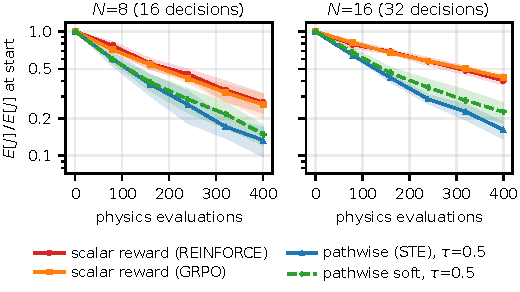
\includegraphics[width=\columnwidth]{figures/fig_e1d_race.pdf}
\caption{Expected objective, relative to its value at the uniform
policy, versus physics evaluations, for a factorised design policy trained
with each estimator ($S{=}8$ per step; 5 tasks per $N$; mean $\pm$ sd).}
\label{fig:e1d}\end{figure}


\begin{figure*}[t]\centering
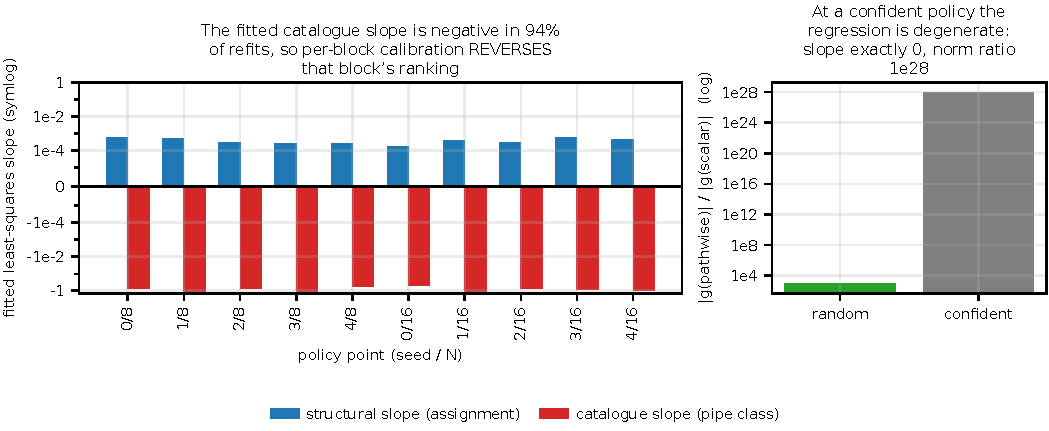
\includegraphics[width=\linewidth]{figures/fig_e1e_calib_slopes}
\caption{Why per-block affine calibration fails on the production solver, and why it fails harder the
better the policy is. \emph{Left}: the least-squares slope fitted for each decision block at 10 policy
points (5 seeds $\times$ $N\in\{8,16\}$), 24 independent refits each. The structural slope is positive and
small ($+3.80\times10^{-4}$ median) while the catalogue slope is \textbf{negative in 94\% of refits}
($-0.886$ median). Per-block calibration therefore reverses the catalogue ranking instead of rescaling it.
Under the unit-normalised step a race takes, a global scale cancels, so only this relative weighting and
the two signs survive. \emph{Right}: the pathwise-to-score-function gradient-norm ratio by policy confidence. At a
confident policy all $S$ samples decode to the same design, and the per-sample spread the slope is fitted from
collapses.  Both fitted slopes return exactly $0.0$ at a norm ratio of $10^{28}$: regression-based
calibration is undefined precisely where a converged design agent lives.}
\label{fig:bcalib}
\end{figure*}
\cref{fig:bcalib} exposes a second and more fundamental limitation:
at a \emph{confident} policy point the regression is degenerate. All $S$ samples decode to the same design, and the per-sample variance the slope is
fitted from collapses to zero.  Both fitted slopes return exactly $0.0$.  The
pathwise-to-score-function norm ratio there is $10^{28}$ for the structural block. Regression-based calibration of a pathwise estimator against a score-function
estimator is therefore \emph{undefined} precisely where a converged design agent
lives.  That is an argument against the construction itself and not only against our
parameterisation of it.
% source: ddl/case/benchB/E1e_calibration_slopes/loggers/20260914T223127Z_gpuserver/
%         results_e1e_calibration_slopes.json -> summary["random"] {a_z median
%         +3.801e-04, a_b median -8.863e-01, rho_z +0.361, rho_b -0.261,
%         frac_batches_a_b_negative 0.94, n=10 policy points x 24 refits} and
%         summary["confident"] {a_z = a_b = 0, rho = 0, norm_ratio 1.044e+28}.




\subsection{Why per-block calibration fails, and two guarded variants}
The reason calibration fails is now measured rather than asserted.  Refitting
the slope on each of 24 independent batches over ten policy points, the fitted
catalogue slope has median $-0.886$ and is negative in $94\%$ of batches,
against $+3.80\times10^{-4}$ for the structural block.  Per-block calibration
therefore \emph{reverses} the catalogue ranking instead of rescaling it, as
Supplementary Fig.~S2 shows.  Two guarded variants repair that.  A single slope for
the whole vector reaches $0.454\pm0.182$ on the relaxed objective at $N=8$,
where the pathwise arm is lower at $0.417\pm0.176$.  A per-block slope shrunk
toward norm matching and clipped at zero reaches $0.665\pm0.067$ at $N=16$, the
lowest variance in the comparison, where the pathwise arm is again lower at
$0.642\pm0.204$. It also recovers edit-selection $\rho$ from $-0.113$ to
$+0.401$.  At a confident policy point both slopes are exactly $0.0$ and the
pathwise-to-score-function norm ratio is $10^{28}$, so regression-based
calibration is undefined precisely where a converged design agent lives.
% source: relaxed-objective ratios from
%         ddl/case/benchB/E1b_estimator_types/loggers/20260915T150205Z_race5seed_calibbugfix/
%         results_e1b_lc.json -> summary.race["N8|calib_global"] 0.45403+-0.16314 and
%         ["N16|calib_shrunk"] 0.66453+-0.06002 against ["N8|ste"] 0.41719+-0.15781 and
%         ["N16|ste"] 0.64221+-0.18288 (n = 5; calib_shrunk has the lowest N16 sd of the
%         nine arms).  The superseded values 0.433 and 0.635+-0.032 came from the
%         pre-repair calibration implementation, superseded by the calibbugfix run.

\section{Non-language policy controls}
\label{supp:policies}

\emph{The 6{,}599-parameter factorised policy.}  A factorised policy reading
engineered per-rack physical features was post-trained with the same estimators and
the same \textbf{five} seeds, for 100 steps on a $2{,}000$-step supervised warm
start. The language model ran 200 steps on a 120-step warm start.  It reaches $15.73\pm9.75$ / $9.47\pm8.59$ / $7.86\pm6.63$ at a
training budget of $1{,}600$ forward solves, against $1.08$ / $4.16$ / $7.47$ for the
4B warm start.  Every $\pm$ in this subsection is the sd over seeds with the sample
divisor (ddof=1).  The graph policy trains for 2{,}000 steps on the same
$2{,}000$-step warm start; ratios across policy classes are illustrative rather than
budget-matched.  The language model is
$14.5\times$ better in distribution on validation and $2.3\times$ better on test.
Out of distribution it is not separable from the small policy at five seeds, where
the small policy's own spread ($\pm6.63$ on a mean of $7.86$) is larger than the
difference between the two.
In distribution the gap is a hypothesis-class gap rather than a budget gap: giving
the small policy $15\times$ more physics ($1{,}600\to24{,}000$ solves) leaves
validation plateaus at $11.7$--$15.6$.  Out of distribution the same budgets give
$1.68\to11.33\to0.31$ at two seeds.  That sequence is not monotone, and its endpoint
we do not claim.  This control supports no out-of-distribution ordering above.  At five seeds no paired ordering between the two policies
is claimable.  The exact signed-rank floor at $n=5$ is $p=0.0625$, which never reaches
$\alpha=0.05$ at any effect size.  Six seeds is the smallest count that can.  What
survives is the plateau itself, i.e.\ that the
in-distribution gap is a hypothesis-class gap rather than a budget gap. The estimator ordering inside this control is the cleanest evidence in the paper
for the mechanism itself. One caveat: the score-function arms of this control
carry no reward transform and diverge at every point of a six-point learning-rate
sweep. The ratios measure the divergence of an untransformed baseline rather than
estimator quality; the mechanism evidence rests on the within-invocation
graph-versus-factorised contrast and on the language-model arms.  Pathwise beats
score-function by $169\times$ on validation
regret ($15.73\pm9.75$ against $2665.10\pm558.03$), by $298\times$ on test
($9.47\pm8.59$ against $2818.52\pm617.36$) and by $349\times$ out of distribution
($7.86\pm6.63$ against $2742.96\pm615.07$).  The out-of-distribution ratio is not
separately significant.  All three hold at a comparable budget, on a CPU, in
$9.5$\,s.  The score-function arms do not merely fail to improve: they destroy the shared warm
start.  On validation it goes $21.5\to2665.1$, feasibility is exactly $0.00$, and the
Hamming distance to the reference equals the full slot count on all three splits.  They
collapse to one deterministic infeasible design.
% source: ddl/case/policy/small_policy_posttrain/loggers/20260915T150017Z_matched5/
%         results_small_policy.json (config.seeds = 5, n_params 6599, bench A-v2-20260915,
%         checkvalve / dT_cap 100) -> summary["ste|{val,test,ood}"]
%         {regret_median_mean 15.7251 / 9.4654 / 7.8595, regret_median_all giving ddof=1 sd
%         9.75 / 8.59 / 6.63, total_solves 1600 forward, wall_secs 10.5} and
%         summary["reinforce|{val,test,ood}"].regret_median_mean 2665.10 / 2818.52 / 2742.96
%         (ddof=1 sd 558.03 / 617.36 / 615.07).  The 169x / 298x / 349x are those pairs
%         split by split; no paired test between them is archived, hence "not separately
%         significant".  4B warm start 1.08 / 4.16 / 7.47:
%         ddl/case/analysis/v2A_table/loggers/20260915T163846Z_gpuserver/
%         results_v2A_table.json -> warm_start.{val,test,ood}.regret_median.  Budget
%         plateau (1,600 -> 24,000 solves) and the two-seed ood sequence:
%         loggers/sweep_20260914T195608Z_gpuserver.  Run 20260915T004012Z_matched3
%         (config.seeds = 3) is superseded for every number in this control.
%         ddl/docs/FINDINGS_2026-09-15.md Sec. 13.

\emph{The 16{,}260-parameter graph policy: the hypothesis class is the variable
that mattered.}  The factorised control reads engineered per-rack features.  It cannot
see that two racks in one corridor compete for the same coolant path. A bipartite rack/corridor graph policy with a two-layer pair head was post-trained
in the same process from the same shared warm start, with the same estimators, the
same budget and \textbf{five} seeds.  It reaches $2.25\pm1.66$ / $0.68\pm0.77$ / $1.09\pm0.69$ against the factorised
policy's $13.33\pm6.09$ / $5.74\pm3.47$ / $6.77\pm4.28$ within the same pinned
invocation: $5.92\times$ / $8.41\times$ / $6.20\times$, with exact paired Wilcoxon
$p=0.0035$ / $8.0\times10^{-5}$ / $0.014$.  Against the five-seed factorised runs of a
separate invocation ($15.73\pm9.75$ / $9.47\pm8.59$ / $7.86\pm6.63$) the ratios are
$6.98\times$ / $13.88\times$ / $7.21\times$; the within-invocation values are primary
because the repository's ratio rule forbids crossing invocations.  The
pairing is significant on all three splits.  Every graph-policy number above comes
from an invocation pinned to a single thread, because the policy's aggregation is a
float reduction whose order depends on the thread count. Four pinned invocations
reproduce all eighteen summary cells bit-identically, while unpinned invocations
disagree in nine of eighteen.  Against the
same statistic the five-seed language-model arm of Table~I of the main text records $0.57$ /
$0.32$ / $0.27$. The ordering language model, graph policy, factorised policy
holds within one statistic on all three splits.
% source: the factorised triple is the control's own five-seed run,
%         ddl/case/policy/small_policy_posttrain/loggers/20260915T150017Z_matched5/
%         results_small_policy.json -> summary["ste|{val,test,ood}"].regret_median_mean
%         15.73 / 9.47 / 7.86; that is the single triple this paper uses for the
%         6,599-parameter policy; the 13.33 / 5.74 / 6.77 triple is the in-process
%         factorised arm of the same pinned invocation and is quoted only as such.  Graph-policy triple from
%         ddl/case/policy/GNN_baseline/loggers/20260915T150746Z_gpuserver_pin1/
%         results_gnn_policy.json -> summary["gnn_ste|{val,test,ood}"]
%         {regret_median_mean 2.2514 / 0.6818 / 1.0908, regret_median_sd_sample
%         1.6613 / 0.7652 / 0.6942}.  The 6.98x / 13.88x / 7.21x are those two triples
%         divided split by split.  The Wilcoxon and McNemar p-values beside them are the
%         SAME-PROCESS contrast archived in that pinned run,
%         tests.contrasts[arm_a=gnn_ste, arm_b=mlp_ste] (val 0.0034715, test 7.9968e-05,
%         ood 0.014046; McNemar 0.00031075 / 0.00091052 / 0.189247), where the factorised
%         comparator was retrained inside the invocation and is
%         summary["mlp_ste|{val,test,ood}"].  Re-deriving those paired tests across the
%         two invocations is outstanding with the p-value regeneration pass.  Language-model
%         medians 0.57 / 0.32 / 0.27:
%         ddl/case/analysis/v2A_table/loggers/20260915T163846Z_gpuserver/
%         results_v2A_table.json -> table.ste.{val,test,ood}.mean_of_medians
%         0.5714 / 0.3200 / 0.2672; the superseded 0.58 / 0.57 / 0.26 matched no key.
Its first version underfit badly, at training cross-entropy $1.30$--$1.82$ against
the factorised policy's $0.995$.  Its pair score was a single linear map and so
additive in the two node states, unable to express a rack$\times$corridor
interaction.  The two-layer head gives $0.6150$.  Exact McNemar
on feasibility gives $p=0.00031$ ($23$ tasks gained, $4$ lost) and $0.00091$ ($21$
gained, $4$ lost) in distribution and on test, and $p=0.19$ out of distribution ($14$
gained, $7$ lost).  The $24$-configuration screen behind it is archived and
selected on \emph{training} cross-entropy and then training Hamming distance, never on the comparison metric. The regret ratios above compare the two policies across independent runs, while
the feasibility McNemar and the regret Wilcoxon compare them within the same pinned
process; the two comparisons are deliberately not mixed.

Two properties of this control matter more than the ratio. Its \emph{zero-physics} floor is statistically indistinguishable from the
factorised policy's \emph{post-trained} arm on all three splits ($p=0.47$ / $0.95$ /
$0.71$).  The $1{,}600$ forward solves that the factorised policy spends therefore buy nothing this warm start
does not already have. And against the language model's warm start ($1.08$ / $4.16$ / $7.47$, at zero
physics) it is $2.07\times$ \emph{worse} in distribution but $6.10\times$ better on
test and $6.85\times$ better out of distribution.  That \emph{reverses} the ordering
the factorised policy reports.  That reversal is provisional:
 it compares a post-trained policy against its own warm start, while the matched
five-seed language-model comparison lives in Table~I of the main text under the median statistic. The defensible statement is
narrower and more useful --- no ordering between a language model and a non-language
policy survives a change of hypothesis class --- and the abstract is scoped to say that.
% source: ddl/case/policy/GNN_baseline/loggers/20260915T150746Z_gpuserver_pin1/
%         (authoritative pinned logger; the unpinned loggers agree)
%         results_gnn_policy.json -> summary and tests.contrasts (the tests are IN the
%         artefact now, round-4 N-9), policies.{gnn,mlp}.n_params 16260/6599, config
%         {seeds 5, arms sft/ste/reinforce, sft_steps 2000, threads 1}, torch_num_threads 1,
%         bench A-v2-20260915, bench_config {checkvalve, 100.0}. One invocation, both policy
%         classes in the same process, ddof=1. Screen: loggers/screen_20260915T022500Z_gpuserver.
%         REPRODUCIBILITY, and why this invocation and not the earlier one: the RackGNN
%         aggregates over incident racks and corridors, a float reduction whose ORDER depends
%         on the thread count, and 2000+100 steps amplify it -- a re-run of the earlier
%         invocation at an identical config moved nine of eighteen summary cells (gnn_ste|test
%         1.5718 -> 0.3303, Wilcoxon ood 0.083 -> 0.265) while all nine RackPolicy cells
%         reproduced to +0.0000. The case now pins --threads (default 1) and stamps
%         torch_num_threads and torch_version into the JSON; four pinned threads=1
%         invocations agree on 18 of 18 cells and 9 of 9 contrasts, unpinned ones differ
%         in 9 of 18 (analysis/consistency_inputs f_gnn_spread). Invocations
%         20260915T023242Z and 20260915T072617Z are SUPERSEDED for every gnn_* number; their
%         mlp_* cells still reproduce and row P3 is RackPolicy only. FINDINGS s33.
%         Bootstrap percentile bounds are ORDER-DEPENDENT (bootstrap_ci draws index arrays and
%         takes the median over them): the val bound is [-6.4002,+0.0000] seed-major against
%         [-5.6573,+0.0000] task-major, and test/ood are identical under both. Any quoted
%         interval must name its pairing order; Wilcoxon and McNemar are order-invariant.

\emph{(e) The non-learned references, and what a regret number is worth.}  Seven
arms that learn nothing run on the same $40$ evaluation rows; five are reported here
and the nearest-greedy and underfit-head arms are archived with them.  The two stochastic ones
use five draw seeds and are reported as mean $\pm$ sd over those five draw seeds. Uniform random over the design space gives $296.03\pm135.41$ /
$511.53\pm190.18$ / $565.91\pm153.92$ at feasibility $0.050$ / $0.013$ / $0.000$ for one
solve. Drawing until a design is \emph{legal} gives $1.41\pm1.10$ / $4.38\pm3.86$ /
$23.39\pm11.22$ for $1$--$32$ solves at feasibility $0.463$ / $0.338$ / $0.075$.  That
is \emph{not} better than the language model's warm start in distribution ($1.08$) on
aggregate: it is better on $3$ of the $5$ draw seeds and worse on $2$.  A per-seed
range of $0.75$ to $3.35$ straddles the warm start.  The five deterministic arms are unaffected and
reproduce exactly. A single-step adjoint-guided greedy ranks the candidate edits by the adjoint's
predicted $\Delta\Jobj$, applies the best of three probed edits, and repeats.  It
reaches $0.153$ / $0.097$ / $0.076$ at feasibility $0.69$ / $0.63$ / $0.75$, for
$9.0$--$12.5$ forward plus $2.0$--$2.9$ adjoint solves \emph{per task}.  That is
$7.1\times$ / $42.9\times$ / $98.1\times$ better than that warm start and $126\times$
/ $97.6\times$ / $103.4\times$ better than the factorised policy. Scoring the stored
labels as designs gives exactly $0.0000$ at feasibility $1.000$ on all three splits, which
is the verification that the labels \emph{are} the best-known reference of
Sec.~VI-A of the main text. An alternating master/subproblem decomposition, not a cut-based Benders scheme,
reaches $0.0242$ / $0.0169$ / $0.0385$ for $514$--$1{,}111$ forward solves.  It
attains the proven optimum exactly on $8$ of the $12$ enumerable rows, being at most
$10.67$ above it on the other four.

The honest reading is that a twelve-solve adjoint-guided greedy beats every learned
designer in this paper, so the contribution here is not a better single-task designer. It
is the measurement of when the gradient can be trusted at all. The same adjoint used to \emph{prune} the neighbourhood instead of to rank it gives
feasibility $0.19$ at the exact-adjoint top-1 pruning against the top-8 on
validation.  That is the operational form of the decision-type asymmetry of
Sec.~VII-B of the main text, measured in the inference-search case of the accompanying
repository.  The greedy above
spends about twelve solves per task precisely because it does not trust a first-order
prediction beyond the one edit it verifies.
% source: ddl/case/policy/greedy_and_oracle/loggers/20260915T092629Z_gpuserver/
%         results_greedy_oracle.json -> summary[<arm>|<split>].{regret_median,feasible_rate},
%         rows[].physics, rows[].regret_vs_true, config {seeds 5, rand_draws 32, max_enum 8000},
%         bench A-v2-20260915. All 15 of this case's log.jsonl files carry a done row.
%         N-7: 0.0000 against the proven optimum is a MEDIAN over the 12 enumerable rows and
%         not a per-row universal. rows[].regret_vs_true is exactly 0.0 in 8 of 12 for
%         alternating_decomp (max +10.6723) and non-zero in 9 of 12 for sensitivity_greedy
%         (max +18.6234) against medians 0.0584 / 0.0770, which is why the body quotes
%         medians and claims no universal.

Taken together these five controls say something more specific than "the language
model is unnecessary" and something less comfortable than "it works". The mechanism
this paper is about --- routing a differentiable solver's gradient into an amortised
design policy --- is demonstrated most sharply by a $6{,}599$-parameter model on a
CPU. The language model's advantage is concentrated in \emph{fitting the task-to-design
mapping in distribution}.  On unseen scale the two are not separable at five seeds.
No claim about generalisation to larger $N$ is therefore available to either side. The comparison that matters is therefore not text versus weights but \emph{who
consumes the gradient}.  A search loop may consume it one edit at a time, a model may
consume it as text, or a model whose weights were updated by it may consume zero
physics evaluations per task.
These are not interchangeable, and the ordering is a property of how the
linearisation is consumed rather than of how much information was supplied. Any claim that a \emph{language} model is required must rest on what a factorised
policy over engineered features structurally cannot express: constraints stated in
natural language, and task families whose features were never engineered.  That is
what the out-of-distribution case has to probe. Larger $N$ alone is not that axis: at five seeds the language model and the
factorised policy are tied there.  A change in sequence length is in any case the
wrong probe for a claim about language, because it confounds the interface with the
length the decoder was trained on.


\section{Transfer to constraints stated in English}
\label{supp:e4text}


The three controls above bound what post-training buys on the objective the agent was trained on. They leave one question open, and it is the only question on which a
\emph{language} model is the sole candidate.  Can the agent honour a constraint that
was never a training target and was never engineered as a feature? A factorised policy over local physical features cannot express ``racks R1 and R2 must share a
CDU'' without being retrained with that feature, and an unconstrained search cannot express it at all.

Seven constraint families are generated with exact machine-checkable predicates
over the decoded design, so satisfaction is never judged by reading model output.
They are: shared CDU, distinct CDUs, forbidden CDU, a cap on how many racks one CDU
may serve, and a cap on how many racks may use one pipe class.  The last two are a
group that must share a pipe class, and a minimum number of distinct pipe classes. Each task is tested on three draws of
\emph{two} constraints at once; no training row contains any of these strings. Two arms cannot see the constraint and serve as the chance reference: the
$6{,}599$-parameter policy of Sec.~VII-G of the main text (third control), loading the same trained weights,
and an unconstrained search.  One further arm sees the constraint as a hard predicate
on candidate edits, which is the strong reference. That reference is made strong
deliberately: edits are ranked lexicographically by (violates, predicted $\Delta\Jobj$) rather than
filtered, because the fixed starting design may already violate the constraint and a filter could then
never repair it. Filtering scores $0.500$; the lexicographic search scores $0.825$. An arm that beats a
weak reference has shown nothing.  \Cref{fig:e4text} draws the per-cluster follow
rates of this comparison.

\begin{figure}[t]\centering
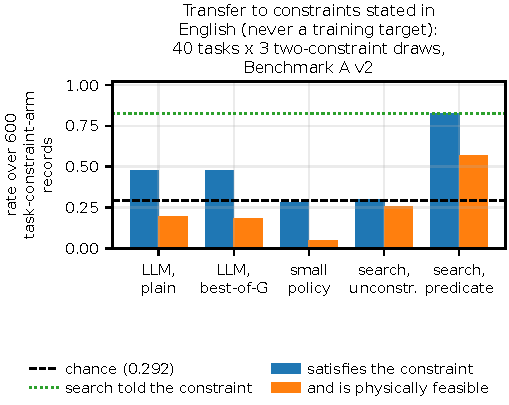
\includegraphics[width=\linewidth]{figures/fig_e4_text_constraints}
\caption{Transfer to constraints stated in English, over 600 task-constraint-arm records (40 tasks
$\times$ 3 two-constraint draws $\times$ 5 arms). Dark bars: the arm's decoded design satisfies the
constraint. Light bars: it satisfies the constraint \emph{and} is physically feasible --- the joint rate,
which is the one that matters, since a legal but unsimulatable design is not a design. The dashed line is
chance, the mean of the two arms that cannot see the constraint at all ($0.292$); the dotted line is a
search handed the same constraint as a hard predicate ($0.825$). The frozen base reaches $0.725$ at one
physics evaluation and the supervised warm start $0.475$; imitation training on design labels costs
$25$ points of compliance.  The $6{,}599$-parameter policy sits at $0.283$, indistinguishable from
chance exactly as its hypothesis class predicts.}
\label{fig:e4text}
\end{figure}
Over $40$ tasks $\times$ $3$ draws, \cref{tab:e4} reports satisfaction and quality
separately:

\begin{table*}[t]\centering\caption{Transfer to held-out ``textual'' constraints, Benchmark~A v2, 40
tasks $\times$ 3 two-constraint draws. ``Both'' is the joint rate: satisfies the constraint ``and''
physically feasible. Regret$|$both is the median regret restricted to tasks where the arm achieved both,
so it measures design quality ``under'' the constraint rather than trading it off against compliance.
The graph policy and the unconstrained search cannot see the constraint and are the chance references}
\label{tab:e4}
\fontsize{7.2}{8.4}\selectfont
\begin{tabular}{@{}lccccc@{}}\toprule
arm & satisfies & feasible & both & regret (med.) & regret$|$both \\
\midrule
\multicolumn{6}{@{}l}{\emph{v2 supervised warm start}}\\
\texttt{LLM, plain prompt} (1 solve) & 0.475 & 0.292 & 0.192 & 4.902 & \textbf{0.0785} \\
\texttt{LLM, best-of-G} (8 solves) & 0.475 & 0.292 & 0.183 & 4.874 & 0.0764 \\
graph policy (1 solve) & 0.283 & 0.225 & 0.050 & 8.932 & 0.2707 \\
\texttt{search, unconstrained} (81) & 0.300 & 0.775 & 0.258 & \textbf{0.0999} & 0.0308 \\
\texttt{search, predicate} (68) & \textbf{0.825} & 0.683 & \textbf{0.567} & 0.1899 & 0.1248 \\
\midrule
\multicolumn{6}{@{}l}{\emph{frozen base, no adapter}}\\
\texttt{LLM, plain prompt} (1 solve) & \textbf{0.725} & 0.283 & 0.192 & 11.220 & 0.3871 \\
\texttt{LLM, best-of-G} (8 solves) & 0.717 & 0.300 & 0.217 & 8.891 & 0.3753 \\
\bottomrule\end{tabular}\end{table*}

\cref{tab:e4} gives the per-arm satisfaction, feasibility and joint rates behind
\cref{fig:e4text}.
% source: ddl/case/llm/E4_ood_transfer/loggers/20260914T225146Z_warmstart and
%         20260914T225146Z_frozenbase -> results_e4_text_constraints.json,
%         summary[<arm>].overall {satisfied_rate, feasible_rate, both_rate, regret_median,
%         regret_median_satisfying, physics_mean}; 600 records per condition.
%         chance level = mean(small_policy 0.283, search_uncon 0.300) = 0.292.

Four things follow.

\emph{The language interface does something no other interface can.} Chance is $0.292$. The frozen base
reaches $0.725$ ($+43.3$ points) and the warm start $0.475$ ($+18.3$ points), at \textbf{one} physics
evaluation. The factorised policy, trained on the same labels, sits at $0.283$ --- indistinguishable from
chance, exactly as its hypothesis class predicts. This is the only measurement we
have that a language model contributes something a smaller model structurally cannot.
% P1-k: the control loaded here is case/policy/small_policy_posttrain/loggers/
%       20260914T224933Z_ckpt/policy_ste_s0.pt -- ONE seed, val 18.40 / test 14.80 / ood 1.33
%       (row P12).  The "regret of 15.6" this sentence used to carry is the TWO-seed scaling run and
%       Sec. VII-F(c) reports the THREE-seed matched3 run (19.27+-6.00), so the number was deleted
%       rather than moved: three invocations, none of them the one whose weights are loaded.
%       Re-running this arm from a matched3 checkpoint is the clean fix and is outstanding.

\emph{And the effect now survives a test that respects its grouping}.  The case
archives all $600$ per-draw records ($5$ arms $\times$ $40$ tasks $\times$ $3$
constraint draws) with the constraint index and the task seed, so an exact test is computable.  Because three draws come from one task, the primary test swaps the two
arms \emph{within} task over $40$ clusters.  An unclustered exact McNemar on the same
$120$ rows is reported beside it; it is anti-conservative in the way
Sec.~VII-D of the main text already records for a pooled count. For the \textbf{frozen base} the advantage over the factorised policy is
significant on validation ($+0.542$, permutation $p=0.0003$) and on test ($+0.375$,
$p=0.0042$).  It is \emph{not} significant out of distribution under the primary test
($+0.375$, Monte-Carlo permutation $p=0.064$ over $8$ clusters, $2\times10^{5}$ draws).  There only the
task-resampled interval $[+0.125,+0.583]$ excludes zero.
The artefact's own rule is that the clustered test governs when the two disagree, so the honest count is
two splits of three, on the weakest interval in the paper.  Against the \emph{other} blind
arm the verdict differs: the unconstrained search is now split-resolved too, and there the
frozen base is significant on all three splits ($+0.479$ at $p=0.00087$, $+0.354$ at
$p=0.0036$, $+0.458$ at $p=0.0398$).  So the out-of-distribution verdict is comparator-dependent: significant against a
search, not significant against a factorised policy.  At $8$ clusters, of which $7$ carry a nonzero
difference, the exact enumeration floor is $0.0156$ and the enumerated two-sided
$p$ is $0.0625$ (the archived Monte-Carlo estimate is $0.0637$ at $2\times10^{5}$
draws). This split therefore cannot reach $0.05$. A sibling invocation whose floors were
computed over pairs rather than clusters is superseded by this one.  ``Every
interface that cannot read it'' is therefore still not established by a single test. For the \textbf{warm start} the pooled effect is significant ($+0.183$ over chance,
interval $[+0.075,+0.292]$; $+0.192$ over the factorised policy, $p=0.016$, interval
$[+0.050,+0.333]$).  It is nonetheless \emph{entirely a validation effect}: on test
the difference is $+0.083$ at $p=0.64$ and out of distribution $+0.042$ at $p=1.00$,
both intervals spanning zero. The alignment tax below is therefore not only a $25$-point level shift: it removes
the significance of the effect on the two held-out splits.  The defensible form of the
claim is that the \emph{untrained} model satisfies an English constraint significantly
better than any interface that cannot read it.  The imitation-trained one does so
only where it was trained. Two limitations travel with this.  One model seed means the clustered test
addresses task grouping and not weight-initialisation variance, which Sec.~VII-D of the main text establishes is real, since the trainer is not run-to-run deterministic.  The control
policy is the single-seed checkpoint noted above.
% source: ddl/case/analysis/e4_significance/loggers/20260915T072042Z_gpuserver/
%         results_e4_significance.json -> comparisons[] {condition, split, difference,
%         cluster_permutation.p, cluster_bootstrap.{ci_low,ci_high}, mcnemar_exact_unclustered}
%         and verdict.txt.  Every published rate was re-derived from the E4 artefact before any test
%         was run on it (reproduction block: 0.475 / 0.2833 / 0.300 / 0.825 / 0.725 / 0.7167 all
%         match to <5e-4).  Primitives are imported from ddl/tools/summarize_runs.py, not reimplemented.

\emph{Imitation training on design labels costs instruction-following.}  The frozen
base satisfies $0.725$; after the supervised warm start the same architecture
satisfies $0.475$, a $25$-point drop.  Its unconstrained design quality meanwhile
improves from regret $11.22$ to $4.90$. That is an alignment tax, measured, on precisely the axis this paper claims is the
language model's reason to exist.  It means the post-training story cannot be told as
monotone improvement, because nothing in the objective rewards constraint compliance.

\emph{A search given the constraint as a predicate beats a model given it in
English}: $0.825$ against $0.475$ on satisfaction and $0.567$ against $0.192$ on the
joint rate, for $68$ solves against $1$.  The gap is significant at $40$ clusters
($p<10^{-4}$, interval $[-0.450,-0.250]$). Against the \emph{frozen} base the same search is ahead by only $0.100$, which is
not significant ($p=0.112$, interval $[-0.208,+0.008]$).  An untuned language model
reading one sentence is statistically indistinguishable from $68$ solves of
constrained local search. Natural
language is expressive enough to state a constraint and not precise enough to enforce it. This is
Sec.~VII-G of the main text from the other direction. There, single-edit sensitivities given as text were read
but not disciplined; here, a whole constraint given as text is understood but not reliably executed.

\emph{Conditional on succeeding, the designs are good, and that is not the binding constraint.} Among tasks
where an arm both satisfies and stays feasible, \texttt{LLM, plain prompt} reaches regret $0.0785$, better than
the constrained search's $0.1248$. The failure is the \emph{joint} rate: $0.192$, so on $80.8\%$ of tasks
the model does not produce a design that is simultaneously legal and physically valid. Separately, constraints are not free.  The unconstrained search reaches regret
$0.0999$ at satisfaction $0.300$, while the constrained one reaches $0.1899$ at
$0.825$.  Honouring the requirement therefore roughly doubles the regret, which is
why satisfaction and quality are never collapsed into one number here.

What this licenses is narrow, and we state it narrowly.  A language-model design
agent can honour a structural constraint it was never trained on and that was never
engineered as a feature, at one physics evaluation.  A $6{,}599$-parameter policy
trained on the same labels sits at chance there. What it does not license is that this beats a constrained search (it is
$1.7\times$ worse on satisfaction and $2.9\times$ worse on the joint rate).  It also
does not license that post-training improves it, since the warm start is $25$ points
worse than the frozen base.  Nor that the resulting designs are usable without
checking.


\section{Reproducibility: task generation, splits and solver constants}
\label{supp:repro}

Every constant needed to rebuild either benchmark is listed here.
Each value is read from the frozen source named beside it, not restated from prose.
\ifblindreview
Benchmark~A is the synthetic solver module of the companion repository, version
\texttt{A-v2-20260915}; its tasks and splits come from the repository's agent and
data scripts and are archived as split files.  Benchmark~B is the companion
repository's liquid-cooling solver over its network generator, version
\texttt{B-lc-20260915}; its splits come from the repository's data script and are
archived likewise.
\else
Benchmark~A is \texttt{ddl/\allowbreak src/\allowbreak thnet.py}, version
\texttt{A-v2-20260915}.
Its tasks and splits come from
\texttt{ddl/\allowbreak src/\allowbreak llm/\allowbreak ddl\_agent/\allowbreak data.py}
and \texttt{ddl/\allowbreak src/\allowbreak llm/\allowbreak make\_data.py}, and are
archived in \texttt{ddl/\allowbreak src/\allowbreak llm/\allowbreak data/\allowbreak bench.json}.
Benchmark~B is \texttt{ddl/\allowbreak src/\allowbreak softlc.py} over the network builder
\texttt{ddl/\allowbreak src/\allowbreak netgen.py}, version \texttt{B-lc-20260915}.
Its splits come from \texttt{ddl/\allowbreak src/\allowbreak lc\_data.py}, and are archived in
\texttt{ddl/\allowbreak src/\allowbreak llm/\allowbreak data\_B/\allowbreak bench.json}.
\fi
Both solvers run in float64.

Both benchmarks minimise one functional form,
\begin{equation}
\begin{split}
\Jobj \;=\;& \frac{P_{\mathrm{pump}}}{100}
\;+\; \lambda_{\mathrm{cost}}\,\mathrm{cost} \\
&+\; \lambda_T \sum_i \bigl(v_{T,i} + v_{T,i}^{2}\bigr)
\;+\; \lambda_Q \sum_k \bigl(v_{Q,k} + v_{Q,k}^{2}\bigr),
\end{split}
\end{equation}
with identical weights on both: $\lambda_{\mathrm{cost}}=0.05$, $\lambda_T=20.0$,
$\lambda_Q=500.0$.
The hinge $v+v^2$ is deliberate, so that a small violation is never cheap.
What differs is the physics, the normalisation of each $v$, and the task draws.
\Cref{tab:reproA} and \cref{tab:reproB} give all three.

\begin{table*}[!t]\centering\caption{Benchmark~A (\rpath{ddl/src/thnet.py}{the companion repository's synthetic solver module}, \texttt{A-v2-20260915}): solver, task-generation and
penalty constants.  \texttt{U}(a,b) denotes one draw from the seeded
\texttt{torch.Generator} of \texttt{random\_task}; draws are independent and taken in the order
listed.  Conductances are in kg$^2$\,s$^{-2}$\,kPa$^{-1}$, so that
$\Delta p=\dot m|\dot m|/C$ is in kPa.  The design variables are the soft assignment
$z\in[0,1]^{N\times K}$ and the soft catalogue $b\in[0,1]^{N\times M}$, both row-stochastic}
\label{tab:reproA}
\fontsize{7.2}{8.4}\selectfont\setlength{\tabcolsep}{4pt}\setlength{\emergencystretch}{1em}
\begin{tabular}{@{}p{0.180\textwidth}p{0.162\textwidth}p{0.560\textwidth}@{}}\toprule
quantity & code name & value \\
\midrule
\multicolumn{3}{@{}l}{\emph{Pipe law, fluid and pump}}\\
pipe law & \texttt{pipe\_flow} & $\dot m=\sqrt{C}\,\Delta p\,/\sqrt{|\Delta p|+\varepsilon_{dp}}$, equivalently $\Delta p=\dot m|\dot m|/C$ \\
law regularisation & \texttt{EPS\_DP} & $\varepsilon_{dp}=1.0\times10^{-3}$\,kPa \\
plate conductance & \texttt{C\_PLATE} & $C_{\mathrm{plate}}=0.02$\,kg$^2$\,s$^{-2}$\,kPa$^{-1}$, fixed and not a decision \\
conductance scale & \texttt{KD} & $K_D=4.0\times10^{6}$; $C_{ik}=C_{\min}+z_{ik}\bigl(K_D\sum_m b_{im}D_m^{5}/L_{ik}-C_{\min}\bigr)$ \\
closure floor & \texttt{C\_MIN\_DEFAULT} & $C_{\min}=2.0\times10^{-5}$\,kg$^2$\,s$^{-2}$\,kPa$^{-1}$ \\
fluid constants & \texttt{RHO}, \texttt{CP} & $\rho=1000$\,kg\,m$^{-3}$; $c_p=4180$\,J\,kg$^{-1}$\,K$^{-1}$ \\
pump efficiency & \texttt{ETA} & $\eta=0.6$ \\
check valve & \texttt{CHECKVALVE\_BETA} & $\beta=50$\,s\,kg$^{-1}$; the curve sees $\tilde m=\mathrm{softplus}(\beta\dot m)/\beta$, i.e.\ $\approx0.02$\,kg/s of smoothing \\
pump curve and balances & \texttt{residual} & $p_k=H_{0,k}\bigl[1-(\tilde m_k/\dot m_{\max,k})^2\bigr]$\,kPa, $\dot m_k=\sum_i\dot m_{ik}$, return manifold at $0$\,kPa, and $\sum_k\dot m_{ik}=\dot m_{\mathrm{plate},i}(p_i)$ per rack \\
Newton solve & \texttt{newton\_solve} & $\le60$ iterations, tolerance $10^{-11}$ on $\max|F|$, $\le20$ backtracking halvings per step \\
\midrule
\multicolumn{3}{@{}l}{\emph{Task draws (\texttt{random\_task}, \texttt{load\_scale}$=1$)}}\\
corridor length & $L_{ik}$ & \texttt{U}(5,40)\,m \\
rack heat load & $q_i$ & \texttt{U}(10,40)\,kW \\
shut-off head & $H_{0,k}$ & \texttt{U}(120,180)\,kPa \\
maximum pump flow & $\dot m_{\max,k}$ & $(N/K)\cdot$\texttt{U}(0.6,1.0)\,kg\,s$^{-1}$ \\
CDU capacity & $Q_{\max,k}$ & $\bigl(\sum_i q_i/K\bigr)\cdot$\texttt{U}(1.1,1.5)\,W; v2 range, v0 used \texttt{U}(0.9,1.4) \\
supply temperature & $T_{\mathrm{sup},k}$ & \texttt{U}(28,32)\,$^\circ$C \\
rack outlet limit & $T_{\lim}$ & $45$\,$^\circ$C, fixed \\
catalogue diameters & $D_m$, $M=3$ & $0.020\,/\,0.030\,/\,0.040$\,m \\
catalogue cost per metre & $c_m$ & $1.0\,/\,1.5\,/\,2.2$ per metre of $L_{ik}$ \\
\midrule
\multicolumn{3}{@{}l}{\emph{Objective terms and normalisations}}\\
pump power & \texttt{P\_pump} & $P_{\mathrm{pump}}=\sum_k \dot m_k p_k\,10^{3}/(\rho\eta)$\,W; enters as $P_{\mathrm{pump}}/100$ \\
pipe cost & \texttt{cost} & $\mathrm{cost}=\sum_{ik}z_{ik}L_{ik}\sum_m b_{im}c_m$, weighted by $\lambda_{\mathrm{cost}}$ \\
rack temperatures & \texttt{evaluate} & $T_{\mathrm{in},i}=\sum_k(\dot m_{ik}/\dot m_i)T_{\mathrm{sup},k}$ and $T_{\mathrm{out},i}=T_{\mathrm{in},i}+q_i/(\dot m_i c_p)$ \\
CDU duty & \texttt{evaluate} & $Q_k=\sum_i q_i\,\dot m_{ik}/\dot m_i$\,W \\
temperature violation & $v_{T,i}$ & $\mathrm{relu}(T_{\mathrm{out},i}-T_{\lim})$ in K, then \texttt{clamp(max=dT\_cap)} at $100$\,K \\
duty violation & $v_{Q,k}$ & $\mathrm{relu}\bigl((Q_k-Q_{\max,k})/Q_{\max,k}\bigr)$, dimensionless \\
frozen bench config & \texttt{BENCH\_CONFIG} & \texttt{pump\_model=checkvalve}, \texttt{dT\_cap=100.0} \\
\midrule
\multicolumn{3}{@{}l}{\emph{Splits (\rpath{ddl/src/llm/data/bench.json}{companion-repository split file})}}\\
counts & \texttt{splits} & train $64$, val $16$, test $16$, ood $8$; $104$ tasks in total \\
sizes, train/val/test & \texttt{sizes} & $(N,K,M)$ cycles $(4,2,3),(6,3,3),(8,3,3)$ with task index $t\bmod 3$ \\
sizes, ood & \texttt{sizes} & $(N,K,M)$ cycles $(12,3,3),(10,2,3)$ \\
seed rule & \texttt{task\_family} & \texttt{seed0}$\,=0$; seed $=$ base $+\,$\texttt{seed0}$\,+t$ with base $10\,000/20\,000/30\,000/40\,000$ \\
oracle labels & \texttt{best\_known} & full-neighbourhood steepest descent plus a coordinate sweep and refine, $5$ shared starts; exhaustive when $(KM)^N\le8000$; $288\,148$ solves total, $2771$ mean \\
\bottomrule\end{tabular}\end{table*}

\begin{table*}[!t]\centering\caption{Benchmark~B (\rpath{ddl/src/softlc.py}{the companion repository's liquid-cooling solver} over \rpath{ddl/src/netgen.py}{its network generator},
\texttt{B-lc-20260915}): friction law, fluid, thermal march, relaxation, penalty and split constants.
\texttt{U}(a,b) denotes one draw from the seeded \texttt{random.Random(seed)} of
\texttt{NG.random\_task}, in the order listed.  Pressures are absolute and in Pa throughout}
\label{tab:reproB}
\fontsize{7.2}{8.4}\selectfont\setlength{\tabcolsep}{4pt}\setlength{\emergencystretch}{1em}
\begin{tabular}{@{}p{0.180\textwidth}p{0.162\textwidth}p{0.560\textwidth}@{}}\toprule
quantity & code name & value \\
\midrule
\multicolumn{3}{@{}l}{\emph{Friction law and hydraulic solver}}\\
friction law & \texttt{pipe\_headloss} & Darcy--Weisbach, $\Delta p=\bigl(fL/D+K\bigr)\dot m|\dot m|/(2\rho A^2)+\rho g\,\Delta h$, with $A=\pi D^2/4$ \\
Reynolds number & \texttt{\_pipe\_dp\_friction} & $Re=\rho v D/\mu$ at $v=|\dot m|/(\rho A)$ \\
friction factor, laminar & \texttt{f\_lam} & $f_{\mathrm{lam}}=64/Re$ \\
friction factor, turbulent & \texttt{f\_turb} & Swamee--Jain, $f_{\mathrm{turb}}=0.25/\bigl[\log_{10}\!\bigl(\varepsilon_r/(3.7D)+5.74/Re^{0.9}\bigr)\bigr]^2$ \\
friction blend & \texttt{sigma} & $f=(1-\sigma)f_{\mathrm{lam}}+\sigma f_{\mathrm{turb}}$ at $\sigma=\mathrm{sigmoid}\bigl((Re-2300)/200\bigr)$ \\
law regularisation & \texttt{eps} & $\varepsilon=10^{-8}$\,kg\,s$^{-1}$ in $|\dot m|=\sqrt{\dot m^2+\varepsilon^2}$ and in every $Re$; $10^{-10}$ added inside $\log_{10}$ \\
roughness and minor loss & \texttt{build\_config} & $\varepsilon_r=1.5\times10^{-6}$\,m; $K=0.5$ per bend \\
device resistance & \texttt{quadratic\_headloss} & $\Delta p=a\,\dot m|\dot m|+b\,\dot m$; cold plate $a=5.0\times10^{5}$, $b=1.0\times10^{4}$; CDU exchanger $a=2.0\times10^{4}$, $b=5.0\times10^{3}$ \\
pump curve & \texttt{pump\_headloss} & $\Delta p=-\rho g\bigl(H_0-a_cQ^2\bigr)n^2$ at $Q=\dot m/\rho$ and $n=1$ \\
hydraulic solve & \texttt{\_HydraulicSolve} & GGA at tolerance $10^{-10}$, $\le60$ iterations, $\dot m_{\mathrm{init}}=0.01$\,kg\,s$^{-1}$ \\
solver fallbacks & \texttt{\_damped\_newton} & damped Newton at tolerance $10^{-9}$, $\le80$ iterations, $\le24$ halvings, residual scales $10^{4}$\,Pa and $10^{-3}$\,kg\,s$^{-1}$; then a homotopy over $t\in\{0.2,0.4,0.6,0.8,1.0\}$ \\
\midrule
\multicolumn{3}{@{}l}{\emph{Fluid, references, thermal march and relaxation}}\\
fluid constants & \texttt{RHO}, \texttt{CP}, \texttt{MU}, \texttt{K\_W\_MK} & $\rho=997$\,kg\,m$^{-3}$; $c_p=4182$\,J\,kg$^{-1}$\,K$^{-1}$; $\mu=8.9\times10^{-4}$\,Pa\,s; $k=0.606$\,W/(m\,K) \\
fixed references & \texttt{T\_SUPPLY\_SECONDARY}, \texttt{T\_LIMIT}, \texttt{P\_REF} & $T_{\mathrm{LIMIT}}=318.15$\,K ($45\,^\circ$C) rack outlet limit; $T_{\mathrm{secondary}}=291.15$\,K ($18\,^\circ$C); $P_{\mathrm{REF}}=1.5\times10^{5}$\,Pa expansion-tank pressure \\
gravity & \texttt{build\_config} & $g=9.81$\,m\,s$^{-2}$ \\
pump efficiency & \texttt{ETA\_PUMP} & $\eta=0.65$ \\
thermal mass-flow floor & \texttt{EPS\_M} & $\varepsilon_m=1.0\times10^{-4}$\,kg\,s$^{-1}$; the march uses $|\dot m|=\sqrt{\dot m^2+\varepsilon_m^2}$, while the friction law uses $10^{-8}$ \\
upwinding form & \texttt{m\_scale} & $w=\mathrm{sigmoid}(\dot m/m_{\mathrm{scale}})$ at $m_{\mathrm{scale}}=5.0\times10^{-3}$\,kg\,s$^{-1}$; an edge delivers $|\dot m|w$ to its head node and $|\dot m|(1-w)$ to its tail node \\
exchanger closure & \texttt{thermal} & NTU effectiveness $\epsilon=1-\exp\!\bigl(-UA/(|\dot m|c_p)\bigr)$, so $T_{\mathrm{out}}=(1-\epsilon)T_{\mathrm{in}}+\epsilon T_{\mathrm{secondary}}$ \\
closure floor & \texttt{C\_MIN} & $C_{\min}=1.0\times10^{-5}$, dimensionless; $w_{ik}=C_{\min}+z_{ik}(1-C_{\min})$ divides both $L$ and $K$ of a branch \\
diameter relaxation & \texttt{relax\_diam} & \texttt{resistance}: $D_i=\bigl(\sum_m p_{im}D_m^{-5}\bigr)^{-1/5}$ \\
catalogue and cost & \texttt{DIAM\_CATALOGUE} & $0.020\,/\,0.028\,/\,0.040$\,m at $11.0\,/\,19.0\,/\,34.0$ per metre \\
\midrule
\multicolumn{3}{@{}l}{\emph{Objective terms and normalisations}}\\
pump power & \texttt{evaluate} & $P_{\mathrm{pump}}=\sum_{\text{pumps}}|\dot m|\,|\Delta p|/(\rho\eta)$\,W; enters as $P_{\mathrm{pump}}/100$ \\
pipe cost & \texttt{evaluate} & $\mathrm{cost}=\sum_{ik}z_{ik}L_{ik}\cdot 2\cdot\sum_m p_{im}c_m$, the factor $2$ being supply and return \\
temperature violation & $v_{T,i}$ & $\max\bigl(T_{\mathrm{out},i}-T_{\mathrm{LIMIT}},0\bigr)/5.0$, in kelvin \\
temperature term is unclamped & \texttt{evaluate} & there is no upper cap: no \texttt{dT\_cap} exists on Benchmark~B, so $v_{T,i}$ and $v_{T,i}^2$ grow without bound \\
duty violation & $v_{Q,k}$ & $\max\bigl(\mathrm{duty}_k-Q_{\max,k},0\bigr)/1000$ in W, at $\mathrm{duty}_k=|\dot m|c_p\bigl(T_{\mathrm{hx,in}}-T_{\mathrm{hx,out}}\bigr)$ \\
solver-failure charge & \texttt{SOLVER\_FAIL\_J} & $10^{9}$, finite, counted and never dropped \\
\midrule
\multicolumn{3}{@{}l}{\emph{Task draws (\texttt{NG.random\_task}) and geometry}}\\
rack heat load & \texttt{loads\_W} & \texttt{U}(6000,26000)\,W per rack \\
CDU rated capacity & \texttt{cdu\_Qmax\_W} & $Q_{\max,k}=\bigl(\sum_i q_i/K\bigr)\cdot$\texttt{U}(1.15,1.55)\,W \\
exchanger UA & \texttt{cdu\_UA} & $UA_k=\bigl(Q_{\max,k}/9.0\bigr)\cdot$\texttt{U}(0.9,1.2)\,W\,K$^{-1}$ \\
shut-off head & \texttt{pump\_H0} & \texttt{U}(22,30)\,m \\
pump curve coefficient & \texttt{pump\_a} & \texttt{U}($0.7\times10^{6}$,$1.4\times10^{6}$)\,s$^{2}$\,m$^{-5}$ \\
floor-plan layout & \texttt{rack\_xy}, \texttt{cdu\_xy} & rack $i$ at $\bigl(1.2i+$\texttt{U}($-0.3,0.3$)$,\;9.0+$\texttt{U}($-1.0,1.0$)$\bigr)$\,m; CDU $k$ at $\bigl(4.0k+$\texttt{U}($-0.5,0.5$)$,\;0\bigr)$\,m \\
branch length & \texttt{branch\_len} & $L_{ik}=\max\bigl(2.0,\;\lVert x_i-x_k\rVert\bigr)$\,m, charged once each to supply and return \\
cold-plate thermal data & \texttt{build\_config} & $UA=4000$\,W\,K$^{-1}$, $C_{\mathrm{solid}}=8000$\,J\,K$^{-1}$, $V_{\mathrm{fluid}}=2.0\times10^{-4}$\,m$^{3}$ \\
\midrule
\multicolumn{3}{@{}l}{\emph{Splits (\rpath{ddl/src/llm/data\_B/bench.json}{companion-repository split file})}}\\
counts & \texttt{splits} & train $48$, val $16$, test $16$, ood $8$; $88$ tasks, feasible rate $1.00$ on every split \\
$N$ range & \texttt{N\_range} & $N\in[6,10]$ on train, val and test, cycled as $N=6+(\mathrm{seed}-\texttt{seed0})\bmod 5$ \\
ood $N$ range & \texttt{ood\_N\_range} & recorded as $[6,10]$, so the shipped ood split is not a scale extrapolation; the \texttt{make\_dataset} default $(12,16)$ was not used \\
$K$ and $M$ & \texttt{bench.json} & $K=3$ CDUs and $M=3$ catalogue classes on every split \\
seed rule & \texttt{make\_dataset} & \texttt{seed0}$\,=900\,000$, contiguous across splits: train $900\,000$--$900\,047$, val $900\,048$--$900\,063$, test $900\,064$--$900\,079$, ood $900\,080$--$900\,087$ \\
oracle labels & \texttt{oracle\_label} & full-neighbourhood steepest descent on the hard compile, $4$ starts, budget $1200$ ($300$ per start); mean $237$--$243$ solves used \\
\bottomrule\end{tabular}\end{table*}

\ifblindreview
The artefact map naming every logged run is provided in the open version of this supplementary.
\else
\emph{Artefact map.}  Every object of the main text and of this supplementary is
reproduced by exactly one logged run.
Paths below are relative to \texttt{ddl/case/}, and each names the logger directory
the manuscript already cites beside the object.

\begingroup\fontsize{7.2}{8.8}\selectfont\raggedright\setlength{\leftskip}{0.6em}\noindent
\texttt{tab:closure} $\leftarrow$ \texttt{benchB/\allowbreak E0f\_closure\_repair}, \texttt{loggers/\allowbreak 20260915T201056Z\_gpuserver}.\\
\texttt{fig:lcclosure} $\leftarrow$ \texttt{benchB/\allowbreak E0c\_field\_snapshots}, \texttt{loggers/\allowbreak 20260915T100812Z\_gpuserver}.\\
\texttt{fig:fields} and \texttt{fig:galleryS} $\leftarrow$ \texttt{benchB/\allowbreak E0d\_case\_gallery}, \texttt{loggers/\allowbreak 20260915T110608Z\_gpuserver}.\\
\texttt{tab:e2} $\leftarrow$ \texttt{analysis/\allowbreak v2A\_table}, \texttt{loggers/\allowbreak 20260915T175120Z\_gpuserver}.\\
main-text Sec.~VII-E $\leftarrow$ \texttt{analysis/\allowbreak v2B\_table}, \texttt{loggers/\allowbreak 20260915T175127Z\_gpuserver}.\\
\texttt{fig:e0} $\leftarrow$ \texttt{benchA/\allowbreak E0\_adjoint\_and\_edits}, \texttt{loggers/\allowbreak 20260914T224553Z\_v2}.\\
\texttt{fig:bedit} $\leftarrow$ \texttt{benchB/\allowbreak E1d\_edit\_ranking}, \texttt{loggers/\allowbreak 20260915T150207Z\_edit5seed}.\\
\texttt{tab:split} $\leftarrow$ \texttt{benchB/\allowbreak E0b\_split\_decision\_type}, \texttt{loggers/\allowbreak 20260916T012509Z\_gpuserver}.\\
\texttt{fig:bcalib} $\leftarrow$ \texttt{benchB/\allowbreak E1e\_calibration\_slopes}, \texttt{loggers/\allowbreak 20260914T223127Z\_gpuserver}.\\
supplementary S-III (\texttt{supp:e4text}) $\leftarrow$ \texttt{analysis/\allowbreak e4\_significance}, \texttt{loggers/\allowbreak 20260915T072042Z\_gpuserver}.
\par\endgroup
\fi

\section{Design trajectory plate}
\label{supp:traj}

\begin{figure*}[!t]\centering
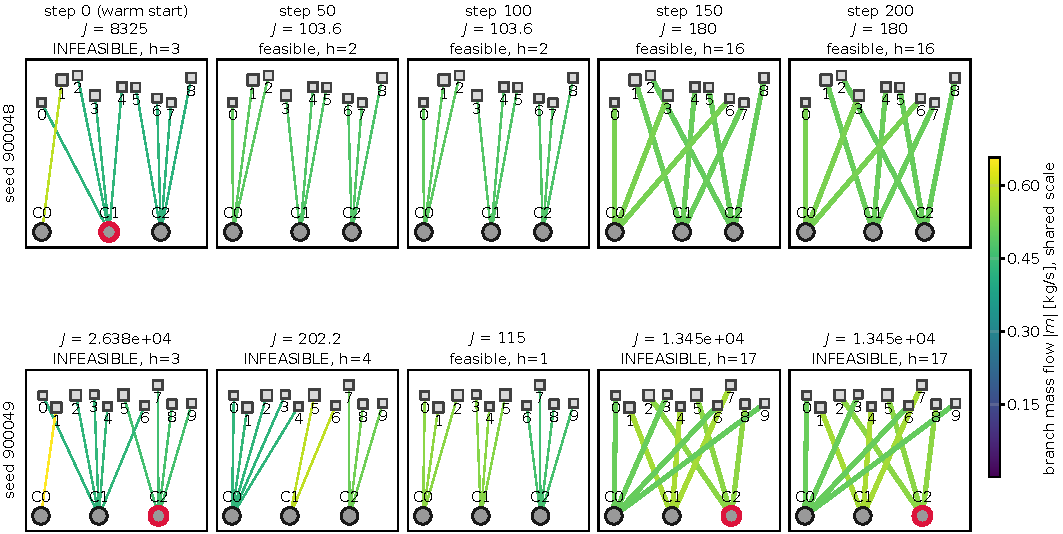
\includegraphics[width=\linewidth]{figures/design_trajectory.pdf}
\caption{One pathwise run at five checkpoints on four tasks: the design the agent emits while it
trains, with its deployed objective, feasibility and Hamming distance to the label.  Feasibility
arrives by step 50 on three of four tasks and is lost again by step 200 on two of them, while the
distance to the label grows from 2--5 decisions to 9--17.  No row is best at its endpoint: the visual form of this subsection's quantitative claim.}
\label{fig:traj}\end{figure*}
\cref{fig:traj} draws one run at five checkpoints before any of it is aggregated.